%\clearpage
\pagebreak
\thispagestyle{empty}

\movetooddpage
\small\textlt
\label{colaboradores}

\noindent{}SOBRE O AUTOR\\
{\small

Aleksei Tolstói (1883--1945), da família do conde Nikolai Tolstói,
nasceu em uma cidadezinha na província de Samara e virou um conhecido e
influente escritor na União Soviética, principalmente a partir da década
de 1930. Aventurou-se por vários gêneros: foi autor de obras realistas e
históricas, como a trilogia \emph{O caminho dos tormentos} (1921--1940) e
o romance histórico inacabado \emph{Pedro \textsc{i}} (1930--1934), e de livros de
ficção científica, como \emph{Aelita} (1923) e \emph{O hiperboloide do
engenheiro Gárin} (1927). Escreveu também para jovens e crianças e
assinou uma adaptação de \emph{Pinóquio} que se tornou conhecida na
Rússia inteira: \emph{A chave de ouro ou as aventuras de Buratino}
(1936).

Foi em Paris, em 1920, que Tolstói começou a publicar \emph{A infância
de Nikita}, nos números 2, 3, 4, 5 e 6 da revista infantil \emph{Varinha
verde.} No entanto, o livro só saiu integralmente em Berlim pela editora
\emph{Guelikon} (1922) com um novo título: \emph{Uma novela sobre muitas
coisas maravilhosas (A infância de Nikita).} Na Rússia, para onde o
autor regressou em 1923, o livro recebeu novamente o título original.

Em 1918 Tolstói, acompanhado por sua terceira esposa, Natália
Krandiévskaia (1888--1963), e por seu filho Nikita, com um ano, saíra dе
Moscou para Odessa. No ano seguinte foram para Constantinopla e então
para Paris, onde Tolstói se envolvera em círculos intelectuais de
emigrados. Quando começou a publicar \emph{A Infância de Nikita},
passava por problemas financeiros e estava isolado artisticamente,
vivendo de pequenas resenhas. Em 1921, partiu para Berlim com a promessa
de dirigir uma revista literária independente.

Marcada pelo tom autobiográfico, \emph{A infância de Nikita} descreve um
ano da vida de Nikita, um garoto de nove anos que morava numa
propriedade rural em Sosnovka, na província de Samara, com a mãe, o pai
e o preceptor, no fim do século \textsc{xix}. O campo, idealizado em Sosnovka, é
um depositório de experiências de iniciação, mediadas por animais, por
fenômenos da natureza e pelas estações do ano.

O desejo de retorno à Rússia --- onde Aleksei Tolstói se tornará um
escritor de renome, o ``Conde Vermelho'' --- é visível na obra, embora
seu conteúdo se afaste das tendências pedagógicas que surgiam na Rússia
de então e se aproxime da tradição russa do século \textsc{xix}.
}


\pagebreak

\noindent{}COLABORADORES\\

\noindent{}MOISSEI MOUNTIAN, nascido na Moldávia (\textsc{urss}), é formado em engenharia civil. Em 1972, mudou"-se com sua esposa, Sofia Mountian, para o Brasil,
onde em 2008 fundou com sua filha Daniela a editora Kalinka e começou a
trabalhar como tradutor. É parte do conselho editorial da Kalinka, tendo
trazido nomes como Fiódor Sologub, Leonid Dobýtchin e Friedrich
Gorenstein aos leitores brasileiros. Foi indicado duas vezes ao Prêmio
Jabuti pelas traduções de {\textltit O diabo mesquinho}, de Fiódor Sologub
(Kalinka, 2008) e {\textltit “Os sonhos teus vão acabar contigo”: prosa,
poesia, teatro}, de Daniil Kharms (Kalinka, 2103, com Aurora Fornoni
Bernardini e Daniela Mountian). Também traduziu {\textltit Encontros com Liz
e outras histórias}, de Leonid Dobýtchin (Kalinka, 2009), {\textltit Diário
de um escritor (1873): Meia carta de um sujeito}, de Fiódor Dostoiévski
(Hedra, 2016), e {\textltit A ressurreição do lariço: Contos de Kolimá 5}, de
Varlam Chalámov (Ed. 34, 2016), os dois últimos em parceria com Daniela.
Com Irineu Franco Perpetuo verteu {\textltit Salmo}, de Friedrich Gorenstein
(indicado ao prêmio de tradução “Lendo a Rússia”, do Instituto de
Tradução de Moscou).

\medskip

\noindent{}IRINEU FRANCO PERPETUO é jornalista, tradutor e crítico de música. Autor, entre outros, de {\textltit História concisa da música clássica brasileira} (Alameda editorial, 2018). Entre suas traduções, consta {\textltit Vida e Destino}, de Vassili Grossman (Ed. Alfaguara, 2014, Prêmio Jabuti de Tradução).

\medskip

\noindent{}FABIO FLAKS \lipsum[12]

\medskip

\noindent{}PAULO HENRIQUE POMPERMAIER é graduado em Jornalismo pela Faculdade Cásper Líbero e graduando em Letras pela \textsc{usp}. Como repórter atuou na Revista {\textltit Cult} e atualmente é editor assistente da Hedra.

\afterpage{\blankpage}

\newpage
\pagestyle{empty}

\tiny{
\noindent{}CATÁLOGO DA EDITORA KALINKA\\[5pt]

\noindent{}O Diabo Mesquinho\\
FIÓDOR SOLOGUB
\medskip

\noindent{}Encontros com Liz e outras histórias\\(Coleção Contos russos modernos, 1900-1930)\\
LEONID DOBÝTCHIN
\medskip

\noindent{}“Os sonhos teus vão acabar contigo”: prosa, poesia, teatro\\(Coleção Contos russos modernos, 1900-1930)\\
DANIIL KHARMS
\medskip

\noindent{}Luminescência: antologia poética\\
VIATCHESLÁV KUPRIYÁNOV
\medskip

\noindent{}Luminescência: desdobramentos\\
VIATCHESLÁV KUPRIYÁNOV
\medskip

\noindent{}Poesia russa: seleta bilíngue
\medskip

\noindent{}Tarakã, o bigodudo (Ars et Vita e Kalinka)\\
KORNEI TCHUKÓVSKI
\medskip

\noindent{}Parque Cultural\\
SERGUEI DOVLÁTOV
\medskip

\noindent{}Salmo\\
FRIEDRICH GORENSTEIN
\medskip

\noindent{}O ofício\\
SERGUEI DOVLÁTOV
\medskip

\noindent{}O elefante (Coleção Mir)\\
ALEKSÁNDR KUPRIN
\medskip

\noindent{}A velha (Coleção Mir)\\
DANIIL KHARMS 
\medskip

\noindent{}Bobók \& ‘Meia carta’ de sujeito (Coleção Mir)\\
FIÓDOR DOSTOIÉVSKI
\medskip

\noindent{}Aulas de literatura russa: de Púchkin a Gorenstein \\
AURORA FORNONI BERNARDINI
\medskip

\noindent{}O compromisso\\
SERGUEI DOVLÁTOV
\medskip

\noindent{}A Cidade Ene (Coleção Contos russos modernos, 1900-1930)\\
LEONID DOBÝTCHIN
\medskip

\noindent{}A infância de Nikita (Coleção Bella)\\
Aleksei Tolstói
}

%\bigskip
\pagebreak


%\newpage
%\begin{center}
%\small
%A Cidade Ene
%
%Город Эн
%\end{center}
%
%\scriptsize
%
%
%\begin{vplace}[1]
%\begin{figure}[!ht]
%%%\begin{minipage}{2\textwidth}
%\centering
%
  %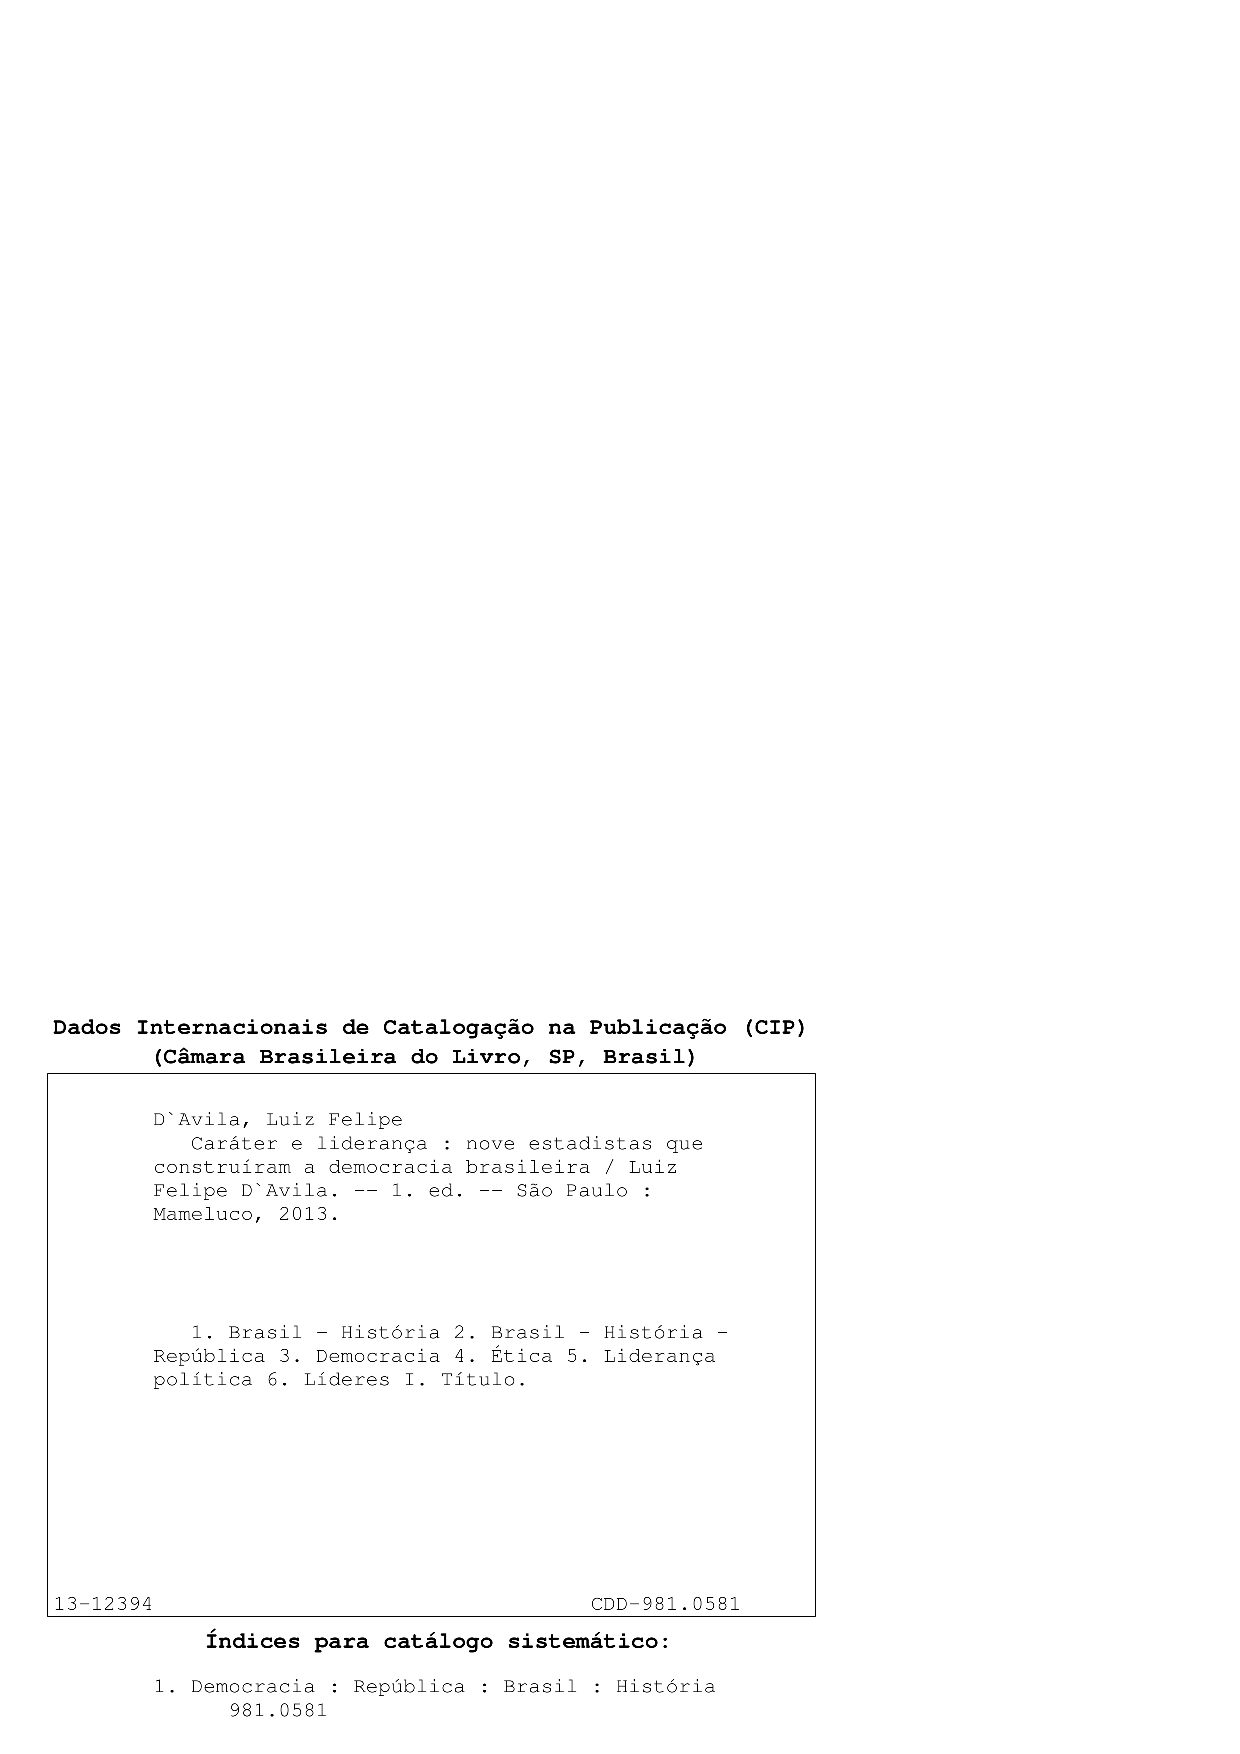
\includegraphics[width=80mm]{./ficha.pdf}
%%%\caption{I}
%%%\end{minipage}
 %\end{figure}
%\end{vplace}

%\begin{vplace}[1]
%\begin{center}
%Dados Internacionais de Catalogação na Publicação (CIP)\\
%(Câmara Brasileira do Livro, SP, Brasil)\\
%\_\_\_\_\_\_\_\_\_\_\_\_\_\_\_\_\_\_\_\_\_\_\_\_\_\_\_\_\_\_\_\_\_\_\_\_\_\_\_\_\_\_\_\_\_\_\_\_\_\_\_\_\_\_\_\_\_\_\_\\
%\end{center}
%\hspace{30pt}Bernardini, Aurora Fornoni, XXXX--


%\hspace{35pt}Aulas de literatura russa : de Púchkin a Gorenstein / Aurora Fornoni

%\hspace{12pt}Bernardini ; organização Valteir Vaz ; prefácio Arlete Cavaliere. - - São Paulo :

%\hspace{12pt}Kalinka, 2018.\\[6pt]

%\hspace{35pt}ISBN XXX-XX-XXXXX-XX-X\\[6pt]

%\hspace{35pt}1. Literatura russa II. Crítica literária III. Título.

%\begin{center}
%\hspace{10pt}XX-XXXXX \hspace{180pt}CDD-XXX.X
%\_\_\_\_\_\_\_\_\_\_\_\_\_\_\_\_\_\_\_\_\_\_\_\_\_\_\_\_\_\_\_\_\_\_\_\_\_\_\_\_\_\_\_\_\_\_\_\_\_\_\_\_\_\_\_\_\_\_\_\\
%Índices para catálogo sistemático:\\[3pt]
%1. Crítica literária : Literatura russa XXX.X\\
%\end{center}
%\end{vplace}
\mbox{}\vfill
\begin{center}
EDIÇÃO: EDITORA KALINKA\\[7pt]
Avenida Angélica, 501 cj. 306\\[7pt]
01227-900 São Paulo-SP Tel.11 2579-6290\\[7pt]
www.kalinka.com.br\\[30pt]

PRODUÇÃO EXECUTIVA: EDITORA HEDRA\\[7pt]
Rua Fradique Coutinho, 1139 Vila Madalena\\[7pt]
05416-011 São Paulo-SP Tel.11 3097-8304\\[7pt]
www.hedra.com.br
\end{center}
%TÍTULO Aulas de literatura russa: de Púchkin a Gorenstein\\
%AUTOR Aurora Fornoni Bernardini\\
%REVISÃO Daniela Mountian e Paulo Henrique Pompermaier\\
%EDIÇÃO Hedra\\
%CAPA Daniela Mountian\\
%PROJETO GRÁFICO Hedra\\
%FORMATO 14 x 21 cm\\
%NÚMERO de PÁGINAS 398\\
%ISBN XXX-XX-XXXXX-XX-X\\